\documentclass[12pt]{article}

\usepackage{amsmath}
\usepackage{amssymb}
\usepackage{geometry}
\usepackage{graphicx}
\usepackage{hyperref}
\usepackage{caption}
\usepackage{subcaption}

\geometry{letterpaper,tmargin=1in,bmargin=1in,lmargin=1in,rmargin=1in}

\hypersetup{
	colorlinks, linkcolor=blue,
}


\begin{document}
	
	\title{Analog IC Design: Project - Part 2}
	\date{Spring 2018}
	\maketitle
	\tableofcontents
	
	\newpage
	\section{Objective}
	
	In part 1 of this project we designed a Operational-Amplifier from scratch. This was done by following a step by step incremental process. This allows for the understanding of each component of the circuit before moving forward to more complicated steps. In continuation of that theme we are going to take that previously constructed circuit and cascade it to increase its overall gain. After that is accomplished we will then attempt to cascade it again but with a single ended output.
	
	\subsection{Primary Tasks}
	The purpose of this project can be simplified into to primary tasks as given.
	\begin{enumerate}
		\item Determining the biasing circuit configuration
		\item Designing/calculate all the MOSFETs parameters to achieve the desired amplifier
		specifications.
	\end{enumerate}
	
	\subsection{Circuit Requirements}
	The following are given circuit requirements that will be adhered to.
	
	\begin{enumerate}
		\item Do whatever modifications necessary to your circuit in the first part to cascode the
		differential stage, as shown in figure 9.13(a) in the textbook.
		\item The new differential gain should be equal to 104
		(with a tolerance of no more than
		20\%, but the gain should be at least 104
		)
		\item Allowed 1 resistor (to be placed outside the IC), any number of n-type and
		p-type enhancement mode MOSFETS.
		\item Allowed a maximum of 2 power supplies (excluding the test input signal source
		of course)
		\item $\lambda$ for all MOSFETS should be at least 0.02
		\item W and L should be at least 1µm (assuming a 1µm technology).
	\end{enumerate}
	
	
	\subsection{Custom MOSFETS}
	\label{sec:desigan_and_analysis}
	
	We will be using the MOSFETs that were designated in part one of the project. They are as follows
	
	\begin{itemize}
		\item NMOS \newline \newline
		.SUBCKT enmos001 1 2 3 \newline
		M 1 2 3 3 enmos001\newline
		.MODEL enmos001 NMOS (KP = 500E-6 VTO = 1 LAMBDA = 0.02 W=2u L=1u)\newline
		.ENDS enmos001
		\newline
		\item PMOS \newline \newline
		.SUBCKT enmos002 1 2 3 \newline
		M 1 2 3 3 enmos002\newline
		.MODEL enmos002 PMOS (KP = 500E-6 VTO = 1 LAMBDA = 0.02 W=2u L=1u)\newline
		.ENDS enmos002
		\newline
		
	\end{itemize}
	
	Using Multisim's component wizard we can import this settings and create custom MOSFETs for use in our simulation.
	
	\subsubsection{Problems Encountered}
	In part one of the project the above MOSFETs where causing wild variations in readings, switching to Multisim 14 helped to solved those problems. Multisim 14 was also used in part two of the project to prevent further issues.
	
	
	\section{Initial Circuit}
	The circuit designed in the previous project is as follows. The sections are colored to show the purpose of each area of the circuit. This is the circuit that will be cascoded for this project. In its current state the gain acheived is 100.
	
	
	\begin{figure}[h!]
		\label{fig:amp}
		\caption{Project: Part 1}
		\centering
		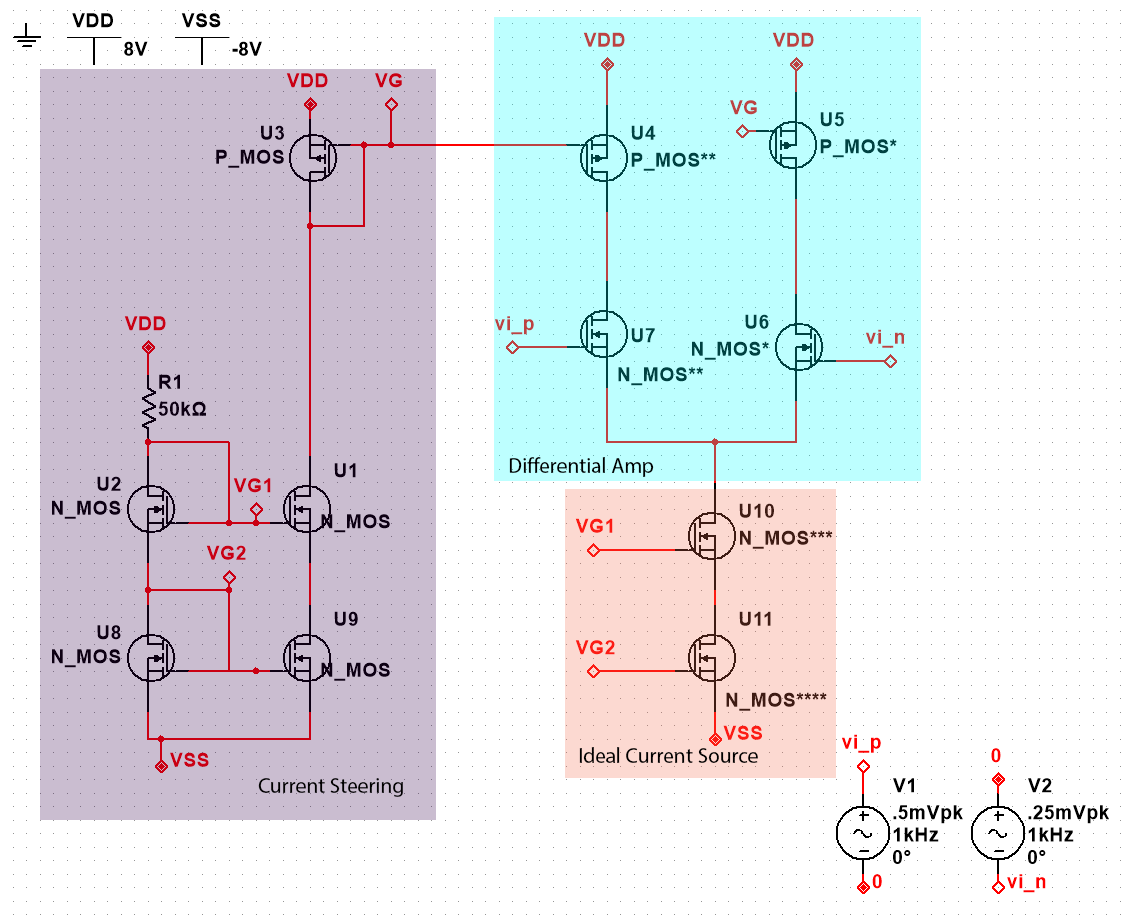
\includegraphics[width=.6\textwidth]{photoshop}
	\end{figure}
	
	
	
	
	\section{Double ended Cascoded Amplifier}
	To design an amplifier to work in a cascoded configuration we must calculate several values, including biasing voltages, drain current, and a new resistance value.
	\subsection{Gain Equation}
	Before we can start solving for other parts of the circuit we need to go ahead and find a equation for the gain of our circuit. From the book we can see that the gain can be obtained by the differential-half circuit of the cascoded amplifier, it is as follows
	
	$$A_d \equiv \frac{V_{od}}{V_{id}} = g_{m1} (R_{on}|| R_{op})$$
	
	where
	$$R_{on} = (g_{m3} r_{o3}) r_{o1}$$ 
	and 
	$$R_{op} = (g_{m5} r_{o5}) r_{o7}$$
	
	with those equations and our equation for transconductance 
	$$g_{m} = \sqrt{2 k_n I_D}$$
	we can begin to solve for $A_D$ knowing that all mosfets have the same parameters.
	
	$$R_{on} =\frac{1}{\lambda I_D} \frac{1}{\lambda I_D} g_m$$
	$$R_{on} = \frac{1}{\lambda^2 I_D^2} g_m$$
	$$R_{on} = \frac{1}{\lambda^2 I_D^2} \sqrt{2 k_n I_D}$$
	$$R_{on}|| R_{op} = \frac{1}{2} \frac{1}{\lambda^2 I_D^2} \sqrt{2 k_n I_D}  $$
	
	Now we take $R_{on}|| R_{op}$ and plug it into our gain equation $A_d \equiv \frac{V_{od}}{V_{id}} = g_{m1} (R_{on}|| R_{op})$
	
	
	$$A_d = \frac{1}{2} \frac{1}{\lambda^2 I_D^2} \sqrt{2 k_n I_D} \sqrt{2 k_n I_D}$$
	which simplifies to our gain equation,
	
	$$A_d  = \frac{k_n}{\lambda^2 I_D}$$
	
	\subsection{Calculating Drain Current $I_d$}
	With the given constants $k_n = k_p = .5m$ and $\lambda = .02$ we can effectively solve for $I_D$ using the gain equation and $A_d = 10000$
	
	$$A_d  = \frac{k_n}{\lambda^2 I_D}$$
	
	
	
	$$I_D = 250\mu A$$
	
	\subsection{Finding Biasing Voltage}
	In order to ensure that all MOSFETs are operating in saturation, we need to find the gate voltage that will cause saturation. We must do this process for both NMOS and PMOS.
	\subsubsection{NMOS Biasing Voltage} 
	Using the current equation 
	$$I_D = \frac{1}{2} k_n (V_G -V_S - V_t)^2 (1 + \lambda V_{ds})$$
	we can solve for $V_G$ using constants and deriving constants. For $V_{DS}$ we will use $V_g + 8$ and for $V_S$ we will use $8v$
	
	$$250 \mu = \frac{1}{2} .001 (V_G + 7)^2 (1+.02(V_G + 8))$$
	 Solving Through gives us 
	 $$0 = .02V_G^3 + 1.44V_G^2 + 17.22V_G + 56.34$$
	 $$V_G = -58, -6.3 , -7.7$$
	 
	 The first value of $V_G$ $-58$ can be immediately disregarded from the extranous solutions due to its extreme variation from the normal values. From simulation the value arrived at is $$V_{Gn} = -6.3V$$ for the bottom biasing NMOS.
	 
	\subsubsection{PMOS Biasing Voltage}
	
	To find the PMOS biasing voltage we go through the same process but using our above value of $V_G$ as our $V_S$. Once resolved the value that we arrive at is
	
	$$V_{Gp} = -5.2V$$
	
	\subsection{Calculating $R_D$}
	We can now find $R_D$ using the values calculated.
	
	$$R_D = \frac{8 + 5.2}{.00025} \approx 53K \Omega$$
	
	\subsection{Current Source $\frac{W}{L}$}
	Knowing that our $W/L$ for each of our branches results in a current of $250 \mu A$ and that it is related directly to current we can double $L$ to obtain an $I$ of $500\mu A$ This results in our current source NMOS to have a ratio of $\frac{4}{1}$
	
	
	\subsection{Circuit Design}
	The final circuit design is as follows. 
		\begin{figure}[h!]
		\label{fig:amp}
		\caption{Project: Part 2 Circuit Design}
		\centering
		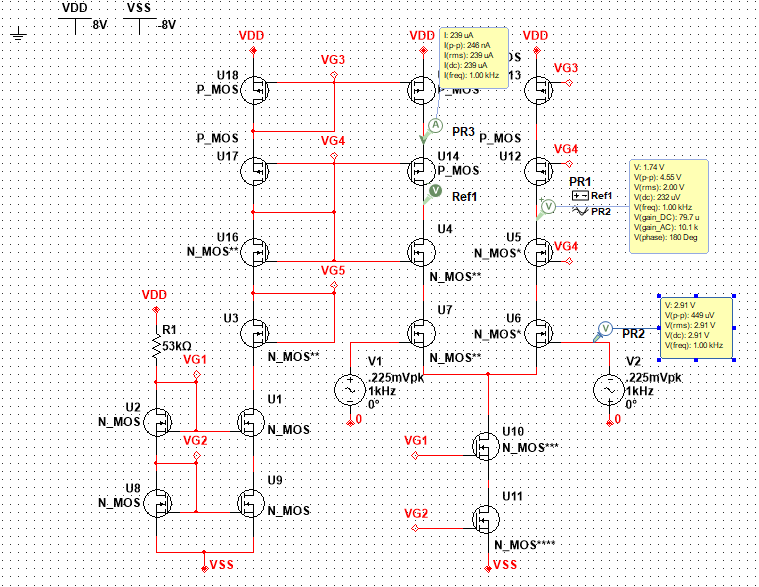
\includegraphics[width=1\textwidth]{fullcircuit}
	\end{figure}

	Each NMOS and PMOS to the left of the cascoded amplifier acts to bias the corresponding MOSFETs on the right. This ensures that all MOSFETs operate in saturation to acheive a correct gain of $\approx 10k$
	
	The NMOS U3 in the figure when connected directly to the small-singal input causes convergence errors, its purpose is to create a biasing voltage for U7, the way that I solved this error is to apply the offset directly to the two input signal as seen in Figure 3. 
	
	
	\begin{figure}
		\centering
		\begin{subfigure}{.5\textwidth}
			\centering
			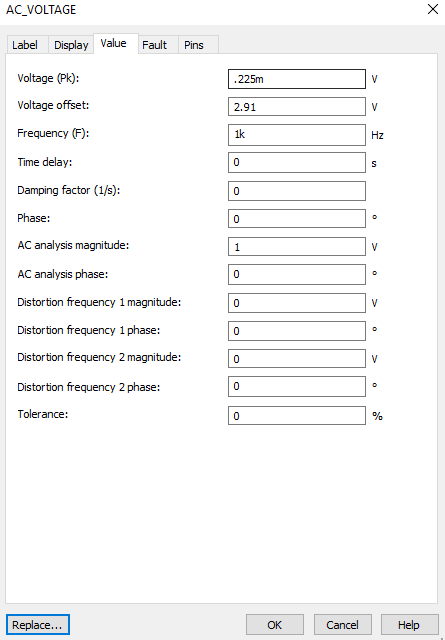
\includegraphics[width=.8\linewidth]{positivebias}
			\caption{Positive Offset}
			\label{fig:sub1}
		\end{subfigure}%
		\begin{subfigure}{.5\textwidth}
			\centering
			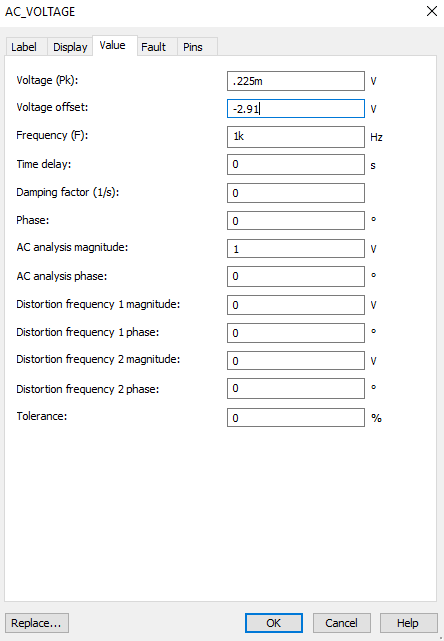
\includegraphics[width=.8\linewidth]{negativebias}
			\caption{Negative Offset}
			\label{fig:sub2}
		\end{subfigure}
		\caption{Offsetting input voltages}
		\label{fig:test}
	\end{figure}
	
	\section{Single-Ended Output }
	Now that we have cascoded out amplifier successfully we can continue our design process to now add another amplifier with a gain of $10$ to a single ended output.
	
	We must also keep in mind that this amplifier because it is single-ended must produce a gain of $20$ that will be reduced by half.
	
	

	\section{Conclusion}
	The project so far has been challenging but rewarding. In terms of progress so far, by chopping the assignment into pieces and individual circuits it made tackling the final circuit that much easier. The Differential amplifier using the given transistors does in fact work, which on its own is very satisfying. I look forward to continuing and completing the design.
	
	
	
	
	
\end{document}
